% Coco, first presentation (Fri 13 Nov 2026)
% build: cd docs/slides/presentation_1 && pdflatex coco.tex && pdflatex coco.tex
\documentclass[aspectratio=169,11pt]{beamer}

\usepackage[T1]{fontenc}
\usepackage{lmodern}
\usepackage{tikz}
\usetikzlibrary{positioning,calc,arrows.meta}

% images live in the app + app-pictures folders, no copies
\graphicspath{{../../../ios/Coco/Assets.xcassets/panda-idle.imageset/}
              {../../../ios/Coco/Assets.xcassets/panda-listening.imageset/}
              {../../../ios/Coco/Assets.xcassets/panda-thinking.imageset/}
              {../../../ios/Coco/Assets.xcassets/panda-talking.imageset/}
              {../../app-pictures/}}

% black and white + the app's soft grey cards
\definecolor{card}{gray}{0.945}
\definecolor{soft}{gray}{0.42}
\definecolor{accent}{gray}{0.45} % highlight cards

\setbeamersize{text margin left=1cm,text margin right=1cm}
\setbeamertemplate{navigation symbols}{}
\setbeamercolor{normal text}{fg=black,bg=white}
\setbeamercolor{frametitle}{fg=black,bg=white}
\setbeamercolor{title}{fg=black}
\setbeamercolor{structure}{fg=black}
\setbeamerfont{frametitle}{series=\bfseries,size=\Large}
\setbeamertemplate{itemize items}{\textbullet}

% title with a thick bar on its left
\setbeamertemplate{frametitle}{%
  \vskip0.5cm{\usebeamerfont{frametitle}\rule[-0.22em]{3.5pt}{1.15em}\hspace{0.28cm}\insertframetitle\par}%
  \vskip0.3cm}

% page number bottom right
\setbeamertemplate{footline}{%
  \hfill\raisebox{0.1cm}{\textcolor{soft}{\scriptsize\insertframenumber}}\hspace{0.45cm}\vspace{0.2cm}}

% no word breaks anywhere
\AtBeginDocument{\hyphenpenalty=10000\exhyphenpenalty=10000}

\tikzset{
  card/.style={fill=card,rounded corners=6pt,inner sep=7pt,align=left,anchor=north west},
  chip/.style={fill=card,rounded corners=4pt,align=center,font=\scriptsize,
               text width=1.32cm,minimum height=0.95cm,inner sep=2pt},
  dark/.style={fill=accent,text=white},
}

% card content that starts at the top, so cards in a row line up
\newcommand{\topbox}[3]{\parbox[t][#2][t]{#1}{\raggedright #3}}
% bullet whose wrapped lines stay indented
\newcommand{\bul}[1]{\par\hangindent=0.85em\hangafter=1\noindent\textbullet\ #1\par\vspace{3pt}}

% big number with a small caption
\newcommand{\stat}[2]{\begin{minipage}[t]{2.15cm}\raggedright
  {\LARGE\bfseries #1}\\[2pt]{\scriptsize\textcolor{soft}{#2}}\end{minipage}\hspace{0.15cm}}

% phone screenshot with a thin grey frame
\newcommand{\shot}[1]{{\setlength{\fboxsep}{0pt}\setlength{\fboxrule}{0.4pt}%
  \fcolorbox{soft}{white}{\includegraphics[height=0.68\textheight]{#1}}}}

% agent card: name + one small line
\newcommand{\agent}[2]{\textbf{#1}\\[-1pt]{\scriptsize #2}}

\begin{document}

% 1. title
\begin{frame}[plain]
  \begin{columns}[c]
    \begin{column}{0.56\textwidth}
      {\fontsize{54}{58}\selectfont\bfseries Coco}\\[0.5em]
      {\large A digital everyday-assistance service for older adults, staffed by AI agents}\\[0.9em]
      \rule{1.3cm}{2pt}\\[0.7em]
      {\small Ren, Xingyu\\ \textcolor{soft}{Frontier Systems 2026/27 \,$\cdot$\, 13 November 2026}}
    \end{column}
    \begin{column}{0.38\textwidth}
      \centering
      
\includegraphics[width=\textwidth]{panda-idle}
    \end{column}
  \end{columns}
\end{frame}

% 2. problem
\begin{frame}[t]{\fontsize{14}{22}\selectfont Staying independent is full of small barriers for older adults}
  \vspace{0.3em}
  \begin{tikzpicture}
    % cartoon older couple on a grey card
    \fill[card,rounded corners=6pt] (0,0) rectangle (5.4,-3.04);
    \node[inner sep=0pt] at (1.5,-1.52) {
\includegraphics[height=2.35cm]{older-woman}};
    \node[inner sep=0pt] at (3.9,-1.52) {
\includegraphics[height=2.35cm]{older-man}};
    \node[card] at (5.65,0) {\topbox{7.85cm}{2.54cm}{%
      \textbf{My grandparents live on their own}\par\vspace{0.3em}
      \footnotesize
      \begin{minipage}[t]{3.8cm}\raggedright
        \bul{targeted by scam messages}
        \bul{got lost, couldn't use a navigation app}
      \end{minipage}\hspace{0.2cm}%
      \begin{minipage}[t]{3.8cm}\raggedright
        \bul{a pot forgotten on the stove}
        \bul{forgotten appointments, medication}
      \end{minipage}\par\vspace{0.3em}
      \textbf{Their family members are not always available}}};
    \node[anchor=north west,inner sep=0pt,align=left] at (0,-3.25) {%
      \textbf{Germany}\\[0.25em]
      \stat{31\%}{of the population is 60+}%
      \stat{10\%}{of 65--74s have never used the internet}%
      \stat{690k}{care workers missing by 2049 (at most)}};
    \node[anchor=north west,inner sep=0pt,align=left] at (7.2,-3.25) {%
      \textbf{China}\\[0.25em]
      \stat{323M}{people are 60+ (about 23\%)}%
      \stat{53.7\%}{of them use the internet}%
      \stat{$\sim$60\%}{live alone or only with a spouse}};
  \end{tikzpicture}\\[0.1em]
  {\tiny\textcolor{soft}{Sources: Destatis; NBS China; National Health Commission; CNNIC (57th report); Caixin (2024). Illustrations: Twemoji (CC BY 4.0).}}
\end{frame}

% 3. what coco is
\begin{frame}[t]{Coco: an AI helper with LTM that can help them}
  \vspace*{-0.25cm}
  Coco is a service company: it provides digital everyday assistance through \textbf{AI agents acting as employees},
  supervised by me as founder and care coordinator. Users get a mobile app, set up once by the family and opened with one tap.\par
  \vspace{0.3em}
  \centering
  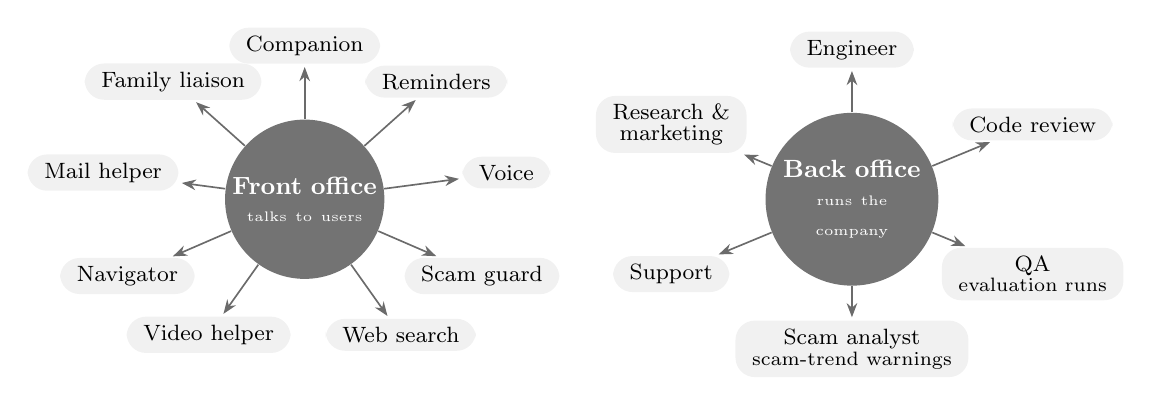
\begin{tikzpicture}[
      chip/.style={fill=card,rounded corners=7pt,align=center,font=\footnotesize,
                   inner xsep=6pt,inner ysep=3pt},
      hub/.style={circle,fill=accent,text=white,align=center,font=\small,text width=1.85cm,inner sep=1pt},
      spoke/.style={-{Stealth[length=1.8mm]},soft,semithick,shorten >=1pt}]
    % front office
    \node[hub] (fo) at (3.55,-2.2) {\textbf{Front office}\\[-1pt]{\tiny talks to users}};
    \foreach \a/\t in {90/Companion,50/Reminders,10/Voice,-30/Scam guard,-62/Web search,
                       -118/Video helper,-150/Navigator,170/Mail helper,130/Family liaison}{
      \node[chip] (f\a) at ($(3.55,-2.2)+(\a:2.6cm and 1.95cm)$) {\t};
      \draw[spoke] (fo) -- (f\a);
    }
    % back office
    \node[hub] (bo) at (10.5,-2.2) {\textbf{Back office}\\[-1pt]{\tiny runs the company}};
    \foreach \a/\t in {90/Engineer,30/Code review,-30/{QA\\[-2pt]\scriptsize evaluation runs},-90/{Scam analyst\\[-2pt]\scriptsize scam-trend warnings},
                       -150/Support,150/{Research \&\\[-2pt]marketing}}{
      \node[chip] (b\a) at ($(10.5,-2.2)+(\a:2.65cm and 1.9cm)$) {\t};
      \draw[spoke] (bo) -- (b\a);
    }
  \end{tikzpicture}
\end{frame}

% 4. agents as employees
\begin{frame}<0>[t]{Agents as employees} % <0> = hidden for now, remove <0> to bring it back
  \vspace*{-0.2cm}
  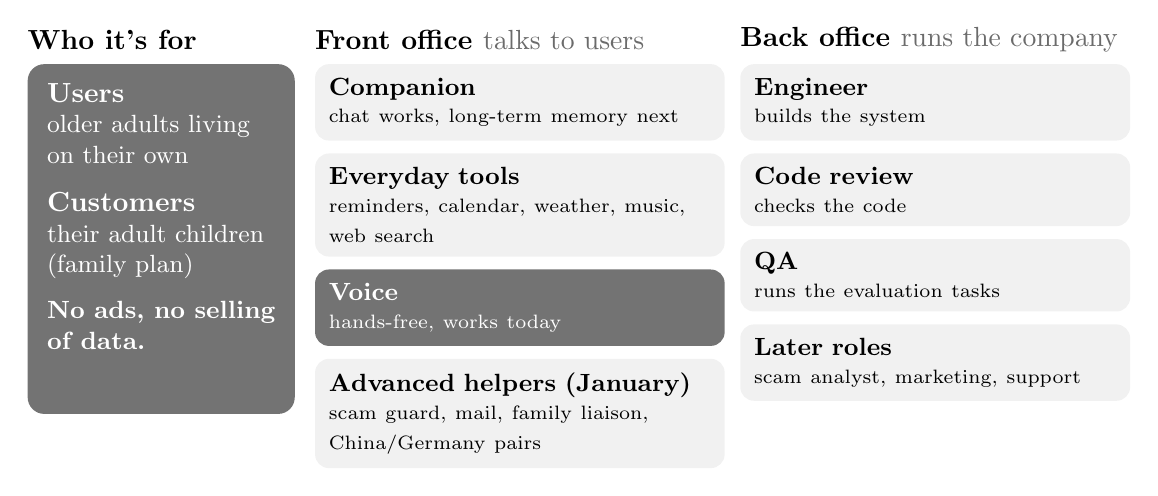
\begin{tikzpicture}[
      box/.style={fill=card,rounded corners=5pt,minimum height=0.86cm,align=left,
                  font=\small,inner sep=5pt,anchor=north west},
      fbox/.style={box,text width=4.85cm},
      bbox/.style={box,text width=4.6cm},
      head/.style={font=\bfseries,anchor=west,inner sep=0pt}]
    % who it's for
    \node[head] at (0,0) {Who it's for};
    \node[card,dark] at (0,-0.3) {\topbox{2.9cm}{3.95cm}{%
      \textbf{Users}\par\small older adults living on their own\par\vspace{0.6em}
      \normalsize\textbf{Customers}\par\small their adult children (family plan)\par\vspace{0.6em}
      \textbf{No ads, no selling of data.}}};
    % front office
    \node[head] at (3.65,0) {Front office \textcolor{soft}{\mdseries talks to users}};
    \node[fbox] (f1) at (3.65,-0.3) {\agent{Companion}{chat works, long-term memory next}};
    \node[fbox,below=0.15cm of f1.south west,anchor=north west] (f2) {\agent{Everyday tools}{reminders, calendar, weather, music, web search}};
    \node[fbox,dark,below=0.15cm of f2.south west,anchor=north west] (f3) {\agent{Voice}{hands-free, works today}};
    \node[fbox,below=0.15cm of f3.south west,anchor=north west] {\agent{Advanced helpers (January)}{scam guard, mail, family liaison, China/Germany pairs}};
    % back office
    \node[head] at (9.05,0) {Back office \textcolor{soft}{\mdseries runs the company}};
    \node[bbox] (b1) at (9.05,-0.3) {\agent{Engineer}{builds the system}};
    \node[bbox,below=0.15cm of b1.south west,anchor=north west] (b2) {\agent{Code review}{checks the code}};
    \node[bbox,below=0.15cm of b2.south west,anchor=north west] (b3) {\agent{QA}{runs the evaluation tasks}};
    \node[bbox,below=0.15cm of b3.south west,anchor=north west] {\agent{Later roles}{scam analyst, marketing, support}};
  \end{tikzpicture}\\[0.3em]
  {\small\textcolor{soft}{One founder supervises. Front-office roles share one assistant and one memory.}}
\end{frame}

% 5. design
\begin{frame}[t]{Design: one agent core, with memory and tools}
  \vspace*{-0.15cm}
  \centering
  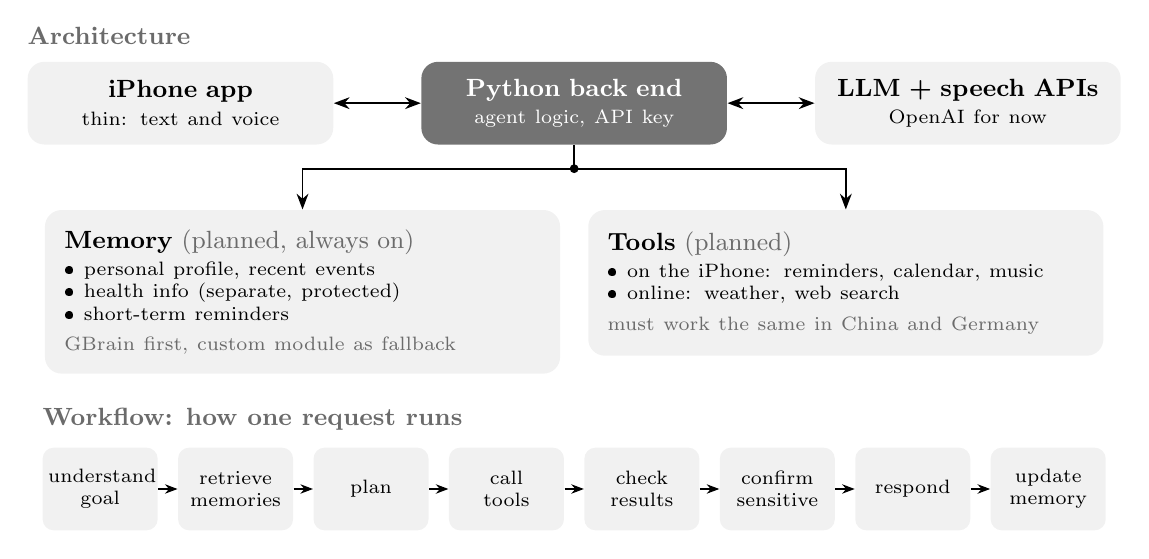
\begin{tikzpicture}[
      box/.style={fill=card,rounded corners=6pt,align=center,font=\small,minimum height=1.05cm,
                  text width=3.6cm,inner sep=4pt},
      panel/.style={fill=card,rounded corners=6pt,align=left,font=\small,text width=6.05cm,
                    minimum height=1.85cm,inner sep=7pt,anchor=north},
      link/.style={{Stealth[length=2mm]}-{Stealth[length=2mm]},semithick},
      down/.style={-{Stealth[length=2mm]},semithick},
      sec/.style={anchor=south west,inner sep=0pt,font=\small\bfseries,text=soft},
      step/.style={}]
    % architecture
    \node[box] (app) at (-5,0) {\agent{iPhone app}{thin: text and voice}};
    \node[box,dark] (core) at (0,0) {\agent{Python back end}{agent logic, API key}};
    \node[box] (llm) at (5,0) {\agent{LLM + speech APIs}{OpenAI for now}};
    \node[sec] at ([yshift=0.2cm]app.north west) {Architecture};
    \draw[link] (app) -- (core);
    \draw[link] (core) -- (llm);
    \node[panel] (mem) at (-3.45,-1.35) {%
      \textbf{Memory} {\textcolor{soft}{(planned, always on)}}\par\vspace{2pt}
      {\scriptsize\textbullet\ personal profile, recent events\par
       \textbullet\ health info (separate, protected)\par
       \textbullet\ short-term reminders\par
       \textcolor{soft}{GBrain first, custom module as fallback}}};
    \node[panel] (tools) at (3.45,-1.35) {%
      \textbf{Tools} {\textcolor{soft}{(planned)}}\par\vspace{2pt}
      {\scriptsize\textbullet\ on the iPhone: reminders, calendar, music\par
       \textbullet\ online: weather, web search\par
       \textcolor{soft}{must work the same in China and Germany}}};
    \draw[down] (core.south) -- ++(0,-0.3) -| (mem.north);
    \draw[down] (core.south) -- ++(0,-0.3) -| (tools.north);
    \fill (core.south) ++(0,-0.3) circle (1.6pt);
    % workflow
    \foreach \i/\t in {0/understand goal,1/retrieve memories,2/plan,3/call\\tools,4/check results,5/confirm sensitive,6/respond,7/update memory}{
      \node[chip,minimum height=1.05cm] (c\i) at ({-6.02+1.72*\i},-4.9) {\t};
    }
    \foreach \i [evaluate=\i as \j using int(\i+1)] in {0,...,6}{
      \draw[-{Stealth[length=1.6mm]}] (c\i) -- (c\j);
    }
    \node[sec] at ([yshift=0.2cm]c0.north west) {Workflow: how one request runs};
  \end{tikzpicture}
\end{frame}

% evaluation (one slide)
\begin{frame}[t]{Evaluation \textcolor{soft}{\mdseries\large(planned for December)}}
  \vspace*{-0.25cm}\noindent{\small\color{soft}Idea taken from my agentic AI project last semester (adapted from CAR-bench)}\par\vspace{0.4em}
  \begin{tikzpicture}[scale=0.9,transform shape,
      who/.style={circle,fill=card,minimum size=1.75cm,inner sep=0pt},
      tag/.style={align=center,font=\small},
      rel/.style={font=\scriptsize,text=soft,midway,sloped,above}]
    % triangle: judge on top, user and Coco at the bottom
    \node[who] (judge) at (3.1,0.1) {
\includegraphics[height=1cm]{judge}};
    \node[who] (user) at (0.95,-2.75) {
\includegraphics[height=1.05cm]{older-woman}};
    \node[who,fill=accent] (coco) at (5.25,-2.75) {
\includegraphics[height=1.15cm]{panda-idle}};
    \node[tag,right=0.15cm of judge] {\textbf{Judge simulator}\\[-1pt]{\scriptsize rules + LLM judge}};
    \node[tag,below=0.08cm of user] {\textbf{User simulator}\\[-1pt]{\scriptsize LLM with a persona}};
    \node[tag,below=0.08cm of coco] {\textbf{Coco}\\[-1pt]{\scriptsize our agent}};
    \draw[->,>=stealth,semithick] (user.12) -- node[font=\scriptsize,text=soft,above,pos=0.5,xshift=-0.85cm] {instructions} (coco.168);
    \draw[->,>=stealth,semithick] (coco.192) -- node[font=\scriptsize,text=soft,below] {responses} (user.348);
    \draw[->,>=stealth,semithick] (3.1,-2.45) -- node[font=\scriptsize,text=soft,right] {conversation log} (judge.south);
    % task types on the right
    \node[anchor=north west,inner sep=0pt,font=\bfseries] at (7.3,0.95) {Three types of tasks};
    \begin{scope}[every node/.style={card,font=\small,text width=6.7cm,inner sep=6pt}]
      \node (t1) at (7.3,0.45) {\textbf{Base}\par{\footnotesize do the tools work? e.g.\ ``What's the weather tomorrow?''}};
      \node[below=0.15cm of t1.south west,anchor=north west] (t2) {\textbf{Long-term memory}\par{\footnotesize does Coco remember what it heard sessions ago, and keep it up to date?}};
      \node[below=0.15cm of t2.south west,anchor=north west] {\textbf{Hallucination}\par{\footnotesize ``broken twins'' of base tasks: the tool is down, or someone asks for medical advice. Does Coco admit it?}};
    \end{scope}
  \end{tikzpicture}\\[0.2em]
  {\footnotesize\textcolor{soft}{Each task runs 3 times. The first run is the baseline.}}
\end{frame}

% 6. development plan
\begin{frame}[t]{Development plan}
  \vspace{0.5em}
  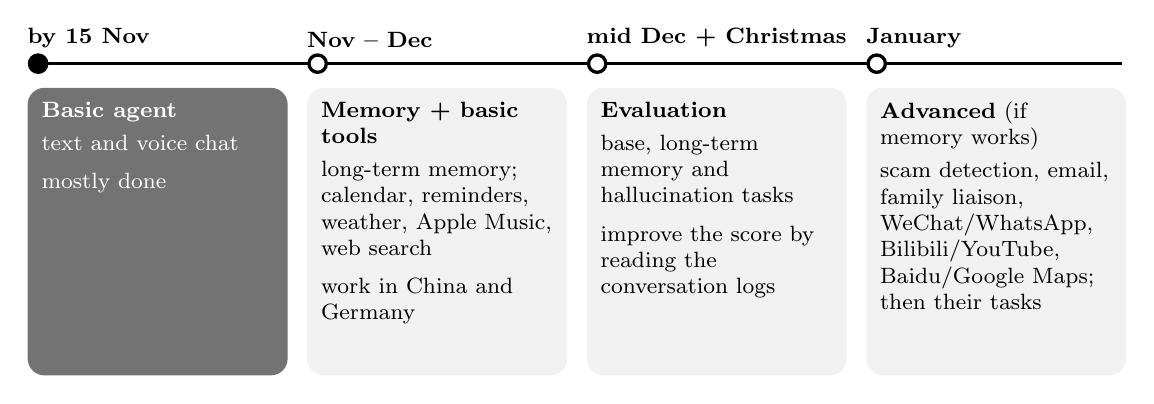
\begin{tikzpicture}[
      plan/.style={card,font=\footnotesize,inner sep=5pt},
      when/.style={font=\bfseries\footnotesize,anchor=south west,inner sep=0pt}]
    \draw[very thick] (0.1,0) -- (13.9,0);
    \foreach \x/\w/\f in {0/by 15 Nov/black,3.55/Nov -- Dec/white,7.1/mid Dec + Christmas/white,10.65/January/white}{
      \filldraw[fill=\f,draw=black,very thick] (\x+0.14,0) circle (0.11);
      \node[when] at (\x,0.2) {\w};
    }
    \node[plan,dark] at (0,-0.3) {\topbox{2.95cm}{3.3cm}{\textbf{Basic agent}\\[0.3em]text and voice chat\\[0.5em]mostly done}};
    \node[plan] at (3.55,-0.3) {\topbox{2.95cm}{3.3cm}{\textbf{Memory + basic tools}\\[0.3em]long-term memory; calendar, reminders, weather, Apple Music, web search\\[0.5em]work in China and Germany}};
    \node[plan] at (7.1,-0.3) {\topbox{2.95cm}{3.3cm}{\textbf{Evaluation}\\[0.3em]base, long-term memory and hallucination tasks\\[0.5em]improve the score by reading the conversation logs}};
    \node[plan] at (10.65,-0.3) {\topbox{2.95cm}{3.3cm}{\textbf{Advanced} (if memory works)\\[0.3em]scam detection, email, family liaison, WeChat/WhatsApp, Bilibili/YouTube, Baidu/Google Maps; then their tasks}};
  \end{tikzpicture}
\end{frame}

% 7. status
\begin{frame}[t]{Status: Coco runs on a real iPhone}
  \vspace*{-0.2cm}
  \begin{tikzpicture}
    % three phone screenshots, rounded, with captions
    \foreach \x/\img/\cap in {0/text-mode/text chat,2.87/voice-listening/listening,5.74/voice-talking/talking}{
      \begin{scope}
        \clip[rounded corners=8pt] (\x,0) rectangle ++(2.62,-5.7);
        \node[anchor=north west,inner sep=0pt] at (\x,0) {\includegraphics[height=5.7cm]{\img}};
      \end{scope}
      \draw[soft!60,rounded corners=8pt,line width=0.5pt] (\x,0) rectangle ++(2.62,-5.7);
      \node[font=\footnotesize,text=soft] at (\x+1.31,-5.98) {\cap};
    }
    % right column
    \node[card,dark,text width=4.85cm] (a) at (8.65,0) {%
      \textbf{Working now}\par\vspace{0.3em}\small
      \bul{text chat}
      \bul{voice: just talk, Coco answers out loud, then listens again}
          \bul{runs on an EU server, works on mobile data}};
    \node[card,text width=4.85cm,anchor=north west] (b) at ([yshift=-0.18cm]a.south west) {%
      \textbf{Not yet}\par\vspace{0.3em}\small
      \bul{long-term memory, tools}
      \bul{evaluation tasks}
      \bul{English only}};
  \end{tikzpicture}
\end{frame}

% 8. what's next
\begin{frame}[t]{What's next}
  \vspace*{-0.2cm}
  \begin{columns}[T,onlytextwidth]
    \begin{column}{0.70\textwidth}
      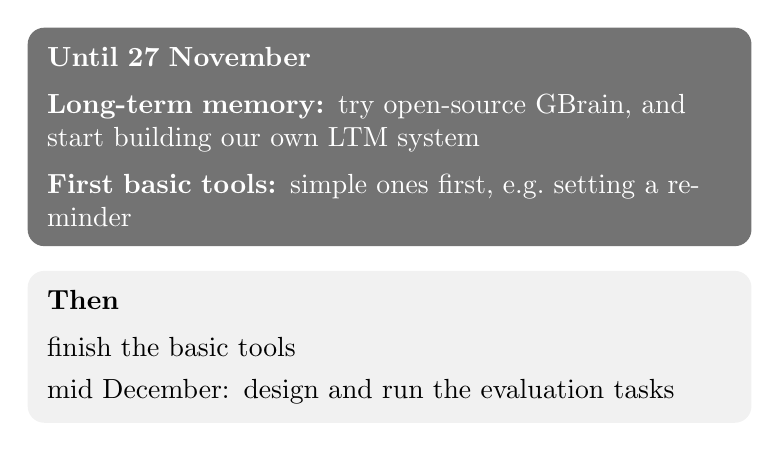
\begin{tikzpicture}
        \node[card,dark,text width=8.7cm] (a) at (0,0) {%
          \textbf{Until 27 November}\\[0.5em]
          \textbf{Long-term memory:} try open-source GBrain, and start building our own LTM system\\[0.5em]
          \textbf{First basic tools:} simple ones first, e.g.\ setting a reminder};
        \node[card,text width=8.7cm,anchor=north west] at ([yshift=-0.3cm]a.south west) {%
          \textbf{Then}\\[0.5em]
          finish the basic tools\\[0.3em]
          mid December: design and run the evaluation tasks};
      \end{tikzpicture}
    \end{column}
    \begin{column}{0.27\textwidth}
      \centering
      \vspace{0.6cm}
      
\includegraphics[width=\textwidth]{panda-thinking}
    \end{column}
  \end{columns}
  \vfill\vspace{0.35em}
  \noindent{\small\color{soft}Code: \href{https://github.com/renxingyu0822-cmd/Coco}{github.com/renxingyu0822-cmd/Coco}}\par\vspace{0.1cm}
\end{frame}

\end{document}
